\chapter{Commitment Tree Generation with internal verification} % (fold)
\label{cha:A Protocol for Commitment Tree Generation}
	
	This chapter describes our approach of creating commitment tree which is built on top of commitment tree generation of SHIA mentioned in the previous chapter.

	\begin{definition}
		\label{def:data-item}
		A commitment tree is a binary tree where each vertex has an associated data-item representing the data that is passed on to its parent. The data-items have the following format:

		$\hspace{100pt}$ $<$id, count, value, commitment$>$\\
		Where id is the unique identity of the node; count is the number of leaf vertices in the subtree rooted at this vertex; value is the SUM aggregate computed over all the leaves in the subtree and commitment is a cryptographic commitment.
	\end{definition}
	There is one vertex $s_{0}$ for each sensor node $s$, which we call the leaf vertex of $s$. 
	\begin{equation}
		\label{eq:leaf-vertex}
		s_{0} = <s_{id}, 1, s_{value}, H(N||1||s_{value})>
	\end{equation}
	\begin{equation}
		Sign(s_{0}) = E_{K_{s}}(H(s_{0}))
	\end{equation}
	In addition to sending the data-item, each sensor node sends the signature of the data-item to its parent.
	The parent node verifies the signature using the child node's public key which is included in child node's certificate.
	After verification of signature it proceeds with the aggregation.
	\begin{definition}
		A \textbf{commitment payload} is a set of data-items of the root of the commitment trees in the outgoing commitment forest.
	\end{definition}

	\textbf{Because of the signature, the sensor node has the proof for the sent data-item.
			It also prevents the parent or ancestor node from claiming the different received data-item.}

	For the given aggregation tree the commitment forest is built as follows.
	Leaf sensor nodes in the aggregation tree creates their leaf vertex according to Equation \ref{eq:leaf-vertex} which they send it to their parent in the aggregation tree.
	Each internal sensor node $s$\ in the aggregation tree also creates their leaf vertex.
	In addition, $s$\ also receives the commitment payload from each of its children which creates the commitment forest for $s$.
	It then merges all the data-items in its commitment forest with same count value to form a new commitment payload.

	Suppose $s$ have to create a commitment payload by merging $i$ data-items $D_{1}$, $D_{2}$, $\dotsc$, $D_{i}$ in its commitment forest.
	First $s$ verifies the signatures $Sign(D_{1})$, $Sign(D_{2})$, $\dotsc$, $Sign(D_{i})$ of $D_{1}$,$D_{2}$,$\dotsc$,$D_{i}$.
	After verification $s$ starts merging the data-items.
	Let $c$ be the smallest count value in the commitment forest.
	The sensor node $s$ finds the two data-items $D_{1},D_{2}$ in the commitment forest with the same count value $c$ and merges them into a new data-item with the count of $c+1$.
	It repeats the process until no two data-items in the forest have the same count value.
	An example of generating the commitment payload by merging the data-items in the commitment forest for the sensor node $A$ in Figure \ref{fig:at} is illustrated in the following example.
	% \ref{fig:commitment-tree-example-1}, \ref{fig:commitment-tree-example-2}, \ref{fig:commitment-tree-example-3}, \ref{fig:commitment-tree-example-4}.
			\begin{exmp} The commitment-payload generation process for node $A$ of Figure \ref{fig:at} is shown here.\\
				\begin{figure}[hp]
					\centering
					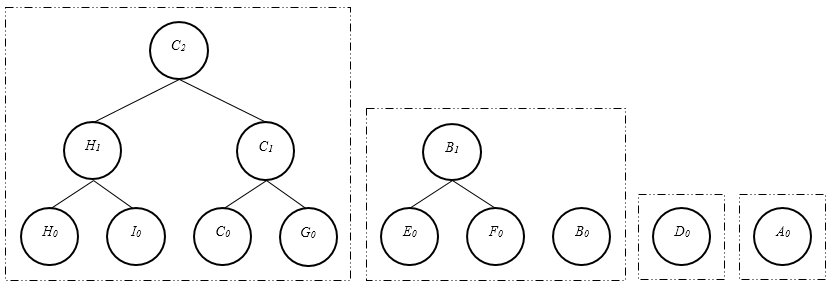
\includegraphics[scale = 1]{images/commitment-tree-example-1.png}\\
					\caption{$A$ receives $C_{2}$ from $C$, $(B_{1},B_{0})$ from $B$, $D_{0}$ from $D$ and generates $A_{0}$. The commitment payload received from a given sensor node is indicated by dashed-line box.}
					\label{fig:commitment-tree-example-1}
				\end{figure}\\
				$A_{0} = <A_{id}, 1, A_{value}, H(N||1||A_{value})>$; $Sign(A_{0}) = E_{K_{A}}(H(A_{0}))$ \\
				$D_{0} = <D_{id}, 1, D_{value}, H(N||1||D_{value})>$; $Sign(D_{0}) = E_{K_{D}}(H(D_{0}))$\\
				$B_{0} = <B_{id}, 1, B_{value}, H(N||1||B_{value})>$; $Sign(B_{0}) = E_{K_{B}}(H(B_{0}))$\\
				$B_{1} = <B_{id}, 2, B_{value}, H(N||2||B_{value}||E_{0}||F_{0})>$; $Sign(B_{1}) = E_{K_{B}}(H(B_{1}))$\\
				$Sign(B_{P}) = E_{K_{B}}(Sign(B_{0}) || Sign(B_{1}))$\\
				$C_{2} = <C_{id}, 4, C_{value}, H(N||4||C_{value})||H_{1}||C_{1})>$; $Sign(C_{2}) = E_{K_{C}}(H(C_{2}))$\\
				\begin{figure}[hp]
					\centering
					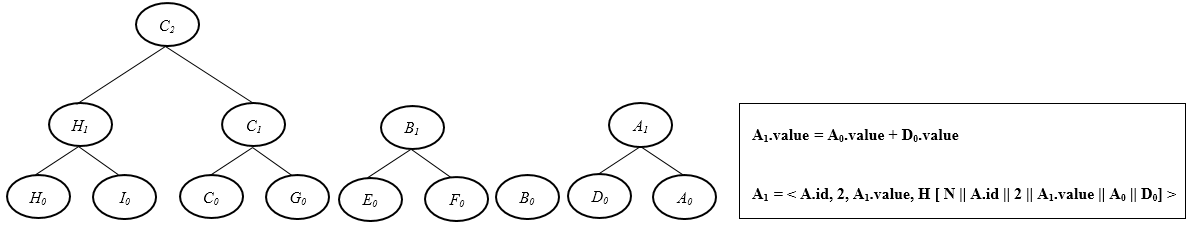
\includegraphics[scale = 1]{images/commitment-tree-example-2.png}\\
					\caption{First Merge: $A_{1}$ vertex created by A.}
					\label{fig:commitment-tree-example-2}
				\end{figure}\\
				$A_{1} = <A_{id}, 2, A_{1value}, H(N||2||A_{1value}||A_{0}||D_{0})>$; $Sign(A_{1}) = E_{K_{A}}(H(A_{1}))$\\
				where $A_{1value} = A_{value} + D_{value} $
				\begin{figure}[hp]
					\centering
					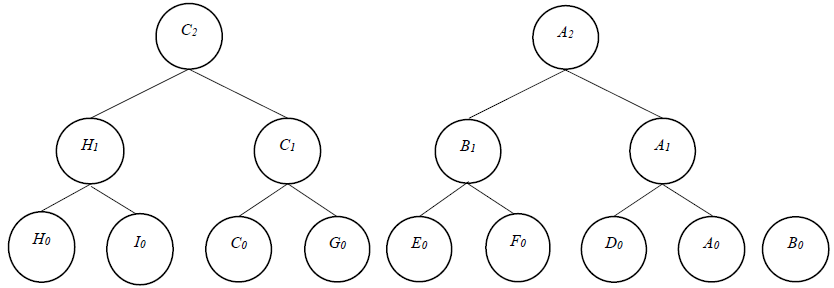
\includegraphics[scale = 1]{images/commitment-tree-example-3.png}\\
					\caption{Second Merge: $A_{2}$ vertex created by A.}
					\label{fig:commitment-tree-example-3}
				\end{figure}\\
				$A_{2} = <A_{id}, 4, A_{2value}, H(N||4||A_{2value}||B_{1}||A_{1}) >$; $Sign(A_{2}) = E_{K_{A}}(H({A_{2}}))$\\
				where $A_{2value} = B_{1value} + A_{1value} $
				\begin{figure}[hp]
					\centering
					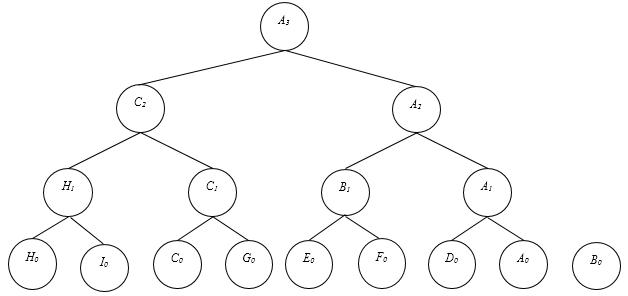
\includegraphics[scale = 1]{images/commitment-tree-example-4.png}\\
					\caption{Third Merge: $A_{3}$ vertex created by A.}
					\label{fig:commitment-tree-example-4}
				\end{figure}\\
				$A_{3} = <A_{id},8, A_{3value},H(N||8||A_{3value}||C_{2}||A_{2})>$; $Sign(A_{3}) = E_{K_{A}}(H(A_{3}))$\\
				$A_{3value} = A_{2value} + C_{2value}$;
			\end{exmp}
% chapter A Protocol for Commitment Tree Generation (end)

Talk about the certificates:
	
	How many certificates does $A$ need to know in this example ?
	In the above example, $A$ need to know $D,B,C's$ certificate to verify their signatures.
	But if we use SHIA'a approach of creating commitment tree then $A$ need to know $E's$ certificate as well.
	Hence, being root in as many tree as possible is the more efficient.
	
